%%%%---------------------------------------------------------------------------------------------------------------
%   PACKAGES
%%%%---------------------------------------------------------------------------------------------------------------

\documentclass[letterpaper,12pt]{book} %two page printing mode
\usepackage{amssymb}
\usepackage{amsmath}
\usepackage{amsfonts}
\usepackage{empheq} %equations environment using amsmath
\usepackage{graphicx}
\usepackage{enumerate}
\usepackage{geometry}
\usepackage{multicol}
\usepackage[ansinew]{inputenc} %auto add accents: ansinew for windwos, latin1 for linux, applemac for macos
\usepackage[spanish]{babel} %spanish words and dashes
\usepackage{verbatim} %use \begin{comment}
\usepackage{amsthm}
\usepackage{mathrsfs}
\usepackage{epsfig}
\usepackage{fancyhdr}
\usepackage{fancybox}
\usepackage{enumitem} %Extended options for List, Numeration and Itemize environments
\usepackage{polynom}
\usepackage{pstricks} %pstricks stuff
\usepackage{pstricks-add} %pstricks stuff
\usepackage{pstricks,pst-node, pst-grad} %pstricks stuff
\usepackage{pstcol} %pstricks stuff
\usepackage{color} %pstricks stuff
\usepackage[labelfont=bf,labelsep=space]{caption} %advanced caption options
\usepackage{float} %activates floating figures
\usepackage[noprefix,refpage,spanish]{nomencl} %symbol list
\usepackage{tocloft} %edit tables names and appearance
\usepackage{centernot} %use to negate log symbols like arcR
\usepackage[none]{hyphenat} %remove hyphenation, use \sloppy to fix overfull lines
\usepackage{bbm} %better R, C, N symbols
\usepackage{textcomp}
\usepackage{nomencl}
\usepackage{mathrsfs}
%%%%---------------------------------------------------------------------------------------------------------------
%   HEADERS AND FOOTERS
%%%%---------------------------------------------------------------------------------------------------------------

\pagestyle{fancy}
\setlength{\headheight}{16pt}
\renewcommand{\chaptermark}[1]{\markboth{\MakeUppercase{#1}}{}}
\fancyhead{} %clear all header fields
\fancyhead[LO]{\textit{N\'UCLEOS POR TRAYECTORIAS MONOCROM\'ATICAS EN DIGR\'AFICAS}}
\fancyhead[RE]{\textit{\leftmark}}
\fancyfoot{} %clear all footer fields
\fancyfoot[CE,CO]{\thepage}
\renewcommand{\headrulewidth}{0.4pt}

%%%%---------------------------------------------------------------------------------------------------------------
%   NAME SWITCHING AND FORMAT
%%%%---------------------------------------------------------------------------------------------------------------

\addto\captionsspanish{\renewcommand{\contentsname}{�ndice}} %\renewcommand{\contentsname}{�ndice} doesn't work, dunno why
\renewcommand{\figurename}{Fig.}
\renewcommand{\proofname}{Demostraci�n}
\renewcommand{\nomname}{�ndice de s�mbolos} %nomenclature shit
\decimalpoint %spanish language interfers with decimal point
\renewcommand{\cftchapdotsep}{4.5} %add dots to index
\renewcommand{\cftfigdotsep}{2} %add dots to figure index
\cftsetindents{figure}{0in}{0.5in} %figure index left side indents

%%%%---------------------------------------------------------------------------------------------------------------
%   THEOREMS
%%%%---------------------------------------------------------------------------------------------------------------

\theoremstyle{plain}
\newtheorem{prox}{Proposici�n}[chapter]
\newtheorem{lemx}[prox]{Lema}
\newtheorem{obsx}[prox]{Observaci�n}
\newtheorem{teox}[prox]{Teorema}
\newtheorem*{teoy}{Teorema} %theorem without number
\newtheorem{defx}{Definici�n}[chapter]
\newtheorem{corox}[prox]{Corolario}
%%%%---------------------------------------------------------------------------------------------------------------
%   MATH SHORTCUTS
%%%%---------------------------------------------------------------------------------------------------------------
\DeclareMathOperator{\arcR}{\longleadsto} %arco
\DeclareMathOperator{\arcL}{\longleftarrow} %arco
\DeclareMathOperator{\arcD}{\longleftleadsto} %arco doble
\DeclareMathOperator{\THEN}{\Rightarrow} %implica
\DeclareMathOperator{\RR}{\mathbbm{R}} %numeros reales
\DeclareMathOperator{\NN}{\mathbbm{N}} %numeros naturales
%\DeclareMathOperator{\CCC}{\mathcal{C}} %
%\DeclareMathOperator{\CCCC}{\mathfrak{C}} %

%%%%---------------------------------------------------------------------------------------------------------------
%   SYMBOL LIST BULLSHIT 
%%%%---------------------------------------------------------------------------------------------------------------

%-------------------------------------------------------
% INSERTAR AQUI TITULO DEL ARCHIVO DE TESIS
%-------------------------------------------------------

\makeindex
\def\execute{%
\begingroup
\catcode`\%=12
\catcode`\\=12
\executeaux}
\def\executeaux#1{\immediate\write18{#1}\endgroup}
\execute{makeindex XENTRIX.nlo -s nomencl.ist -o XENTRIX.nls}
\makenomenclature
\setlength{\nomitemsep}{0.05cm}
\renewcommand{\pagedeclaration}[1]{\dotfill\nobreakspace#1}

%%%%---------------------------------------------------------------------------------------------------------------
%   BRIEF TITLE
%%%%---------------------------------------------------------------------------------------------------------------

\title{N\'ucleos por trayectorias monocrom\'aticas en digr\'aficas}
\author{Jos\'e Mu\~noz Porras}
\date{2011}

%%%%---------------------------------------------------------------------------------------------------------------
%   BEGIN!
%%%%---------------------------------------------------------------------------------------------------------------
\setlength{\headheight}{30.3pt}

\begin{document}
\newrgbcolor{ttqqcc}{0.2 0 0.8}
\newrgbcolor{ffwwqq}{1 0.4 0}
\newrgbcolor{qqttqq}{0 0.2 0}
\newrgbcolor{qqqqzz}{0 0 0.6}
\newrgbcolor{ttttqq}{0.2 0.2 0}
\newrgbcolor{qqqqcc}{0 0 0.8}
\newrgbcolor{zzttqq}{0.6 0.2 0}
\newrgbcolor{xdxdff}{0.49 0.49 1}
\newrgbcolor{ttwwqq}{0.2 0.4 0}
\newrgbcolor{ccqqqq}{0.8 0 0}
\newrgbcolor{ccccqq}{0.8 0.8 0}
\newrgbcolor{ccqqcc}{0.8 0 0.8}
%%%%---------------------------------------------------------------------------------------------------------------
%   COVER + BLANK PAGE
%%%%---------------------------------------------------------------------------------------------------------------


%%%%---------------------------------------------------------------------------------------------------------------
%   TITLE PAGE + BLANK PAGE
%%%%---------------------------------------------------------------------------------------------------------------


%%%%---------------------------------------------------------------------------------------------------------------
%   DATA SHEET (What a shitty piece of code) + BLANK PAGE
%%%%---------------------------------------------------------------------------------------------------------------



%%%%---------------------------------------------------------------------------------------------------------------
%   QUOTE + BLANK PAGE
%%%%---------------------------------------------------------------------------------------------------------------
%%%%---------------------------------------------------------------------------------------------------------------
%   PRELUDE
%%%%---------------------------------------------------------------------------------------------------------------

\frontmatter
\sloppy

%%%%---------------------------------------------------------------------------------------------------------------
%   THANKS
%%%%---------------------------------------------------------------------------------------------------------------

%%%%---------------------------------------------------------------------------------------------------------------
%   TABLE OF CONTENTS
%%%%---------------------------------------------------------------------------------------------------------------


%%%%---------------------------------------------------------------------------------------------------------------
%   INTRODUCTION
%%%%---------------------------------------------------------------------------------------------------------------

\chapter{Introducci�n}
%%%%---------------------------------------------------------------------------------------------------------------
%   THESIS
%%%%---------------------------------------------------------------------------------------------------------------

\mainmatter

%%%%---------------------------------------------------------------------------------------------------------------
%   CHAPTER ONE
%%%%---------------------------------------------------------------------------------------------------------------
\chapter{Definiciones}

Una \emph{gr\'afica dirigida}, o \emph{digr\'afica}, $D$ consiste de un conjunto de v\'ertices no vac\'io y de un conjunto de parejas ordenadas de v\'ertices distintos llamadas flechas. Usaremos la siguiente notaci\'on: \\
Sea $D=(V,A)$ una digr\'afica. $V$ denota el conjunto de v\'ertices y $A$ el de flechas de D. 
\begin{figure}[h!!t]
\begin{center}
\begin{pspicture}(-7.0,-1.86)(8.38,4.3)
\psset{xunit=1.0cm,yunit=1.0cm,algebraic=true,dotstyle=o,dotsize=3pt 0,linewidth=1pt,arrowsize=5pt 2,arrowinset=0.25}
\psline{->}(-1.2,3.4)(0.64,4.72)
\psline{->}(-1.2,3.4)(-0.51,1.24)
\psline{->}(0.64,4.72)(2.46,3.38)
\psline{->}(2.46,3.38)(-1.2,3.4)
\psline{->}(-0.51,1.24)(2.47,3.38)
\psline{->}(0.46,-0.86)(-0.51,1.24)
\psline{->}(2.46,3.38)(1.75,1.23)
\psline{->}(1.75,1.23)(-0.51,1.24)
\parametricplot{1.358652573790421}{3.2160814438036747}{1*1.33*cos(t)+0*1.33*sin(t)+0.16|0*1.33*cos(t)+1*1.33*sin(t)+3.5}
\psdots[dotsize=8pt 0,dotstyle=triangle*,linecolor=blue](0.44,4.8)
\psdots[dotstyle=*,linecolor=blue](0.64,4.72)
\psdots[dotstyle=*,linecolor=blue](-1.2,3.4)
\psdots[dotstyle=*,linecolor=darkgray](-0.51,1.24)
\psdots[dotstyle=*,linecolor=darkgray](1.75,1.23)
\psdots[dotstyle=*,linecolor=darkgray](2.46,3.38)
\psdots[dotstyle=*,linecolor=blue](0.46,-0.86)
\rput[bl](0.72,4.84){\blue{$u$}}
\rput[bl](2.72,3.38){\blue{$v$}}
\rput[bl](-1.62,3.36){\blue{$x_1$}}
\rput[bl](-0.96,1.16){\blue{$x_2$}}
\rput[bl](1.88,0.98){\blue{$x_4$}}
\rput[bl](0.38,-1.2){\blue{$x_3$}}
\end{pspicture}
\caption{Una digr\'afica.}
\label{generada}
\end{center}
\end{figure}

El \emph{orden} de $D$ es el n\'umero de v\'ertices en $D$, es decir, la cardinalidad de $D$. Por ejemplo, el orden de la digr\'afica en la figura 1.1 es 6. \\
Para una flecha $(u,v)$, decimos que $u$ es in-vecino de $v$, o que $u$ es ex-vecino de $v$. Si $(u,v)$ es una flecha tambi\'en decimos que $v$ \emph{absorbe} a $u$, y que  $u$ \emph{domina} a $v$. \\
Sea $D$ una digr\'afica. Una flecha $(u,v)\in A(D)$ es \emph{sim\'etrica} si existe $(v,u) \in A(D)$. Si \emph{todas} las flechas de una digr\'afica $D$ son sim\'etricas, decimos que $D$ es \emph{sim\'etrica}. Si \emph{ninguna} flecha de $D$ es sim\'etrica entonces decimos que $D$ es \emph{asim\'etrica}.  \\
Vamos a utilizar la notaci\'on $[u,v] \in A(D)$ para denotar que $(u,v) \in A(D)$ o que $(v,u) \in A(D)$. \\ 
\begin{figure}[h!!t]
\begin{center}
\begin{pspicture}(-7.0,0)(8.38,5)
\psset{xunit=1.0cm,yunit=1.0cm,algebraic=true,dotstyle=o,dotsize=3pt 0,linewidth=1pt,arrowsize=5pt 2,arrowinset=0.25}
\psline{->}(0.66,4.72)(-1.18,3.4)
\parametricplot{1.358652573790421}{3.2160814438036747}{1*1.33*cos(t)+0*1.33*sin(t)+0.16|0*1.33*cos(t)+1*1.33*sin(t)+3.5}
\psline{->}(1.77,1.23)(2.48,3.38)
\psline{->}(-1.18,3.4)(-0.49,1.24)
\parametricplot{-1.1818394466158892}{0.717083765430057}{1*1.32*cos(t)+0*1.32*sin(t)+1.5|0*1.32*cos(t)+1*1.32*sin(t)+2.52}
\parametricplot{2.5045223243141095}{4.591193057002121}{1*1.24*cos(t)+0*1.24*sin(t)+-0.34|0*1.24*cos(t)+1*1.24*sin(t)+2.5}
\psdots[dotstyle=*,linecolor=blue](0.66,4.72)
\rput[bl](0.66,4.92){\blue{$v$}}
\psdots[dotstyle=*,linecolor=blue](-1.18,3.4)
\rput[bl](-1.42,3.5){\blue{$u$}}
\psdots[dotstyle=*,linecolor=darkgray](-0.49,1.24)
\psdots[dotstyle=*,linecolor=darkgray](1.77,1.23)
\psdots[dotstyle=*,linecolor=darkgray](2.48,3.38)
\psdots[dotsize=4pt 0,dotstyle=triangle*,linecolor=blue](0.44,4.8)
\psdots[dotsize=4pt 0,dotstyle=triangle*,linecolor=blue](2,1.3)
\psdots[dotsize=4pt 0,dotstyle=triangle*,dotangle=90,linecolor=blue](-1.34,3.24)
\end{pspicture}
\caption{Una digr\'afica sim\'etrica.}
\label{generada}
\end{center}
\end{figure}

Dada una digr\'afica $D$, una \emph{subdigr\'afica} de $D$ es la digr\'afica que se forma si tomamos un subconjunto de v\'ertices de D y tomamos todas las flechas que tienen como v\'ertices iniciales o terminales uno de esos v\'ertices. \\
Por ejemplo, la digr\'afica de la Figura 1.3 es subdigr\'afica de la de la Figura 1.2\\. 
Una \emph{digr\'afica inducida} por un conjunto de v\'ertices $V' \subseteq V$, denotada por $D[V']$, es la digr\'afica que tiene como conjunto de v\'ertices a $V'$ y que contiene a todos las flechas que contiene $A$ sobre ese conjunto de v\'ertices. \\ 
\begin{figure}[h!!t]
\begin{center}
\begin{pspicture}(-6.5,2.5)(8.38,5.3)
\psset{xunit=1.0cm,yunit=1.0cm,algebraic=true,dotstyle=o,dotsize=3pt 0,linewidth=1pt,arrowsize=5pt 2,arrowinset=0.25}
\psline{->}(0.66,4.72)(-1.18,3.4)
\parametricplot{1.358652573790421}{3.2160814438036747}{1*1.33*cos(t)+0*1.33*sin(t)+0.16|0*1.33*cos(t)+1*1.33*sin(t)+3.5}
\psdots[dotstyle=*,linecolor=blue](0.66,4.72)
\rput[bl](0.66,4.92){\blue{$v$}}
\psdots[dotstyle=*,linecolor=blue](-1.18,3.4)
\rput[bl](-1.54,3.34){\blue{$u$}}
\psdots[dotsize=8pt 0,dotstyle=triangle*,linecolor=blue](0.44,4.8)
\end{pspicture}
\caption{Una subgr\'afica inducida por un conjunto de v\'ertices.}
\label{generada}
\end{center}
\end{figure}

Una gr\'afica es \emph{completa} si para todo par de v\'ertices $u,v$ existe $(u,v)\in A(D)$. \\
La \emph{gr\'afica subyacente} de una digr\'afica $D = (V,A)$, es la gr\'afica que tiene como conjunto de v\'ertices a V, y $u$ y $v$ son adyacentes, si y solo si, $(u,v)\in A(D)$ o $(v,u) \in A(D)$. \\
Una digr\'afica es \emph{semicompleta} si su gr\'afica subyacente es completa.
\begin{figure}[h!!t]
\begin{center}
\begin{pspicture}(-7,0.86)(8.38,4.5)
\psset{xunit=1.0cm,yunit=1.0cm,algebraic=true,dotstyle=o,dotsize=3pt 0,linewidth=1pt,arrowsize=4pt 2,arrowinset=0.25}
\psline{->}(0.66,4.72)(-1.18,3.4)
\psline{->}(0.66,4.72)(2.48,3.38)
\psline{->}(1.77,1.23)(-0.49,1.24)
\psline{->}(1.77,1.23)(2.48,3.38)
\psline{->}(-1.18,3.4)(-0.49,1.24)
\psline{->}(0.66,4.72)(1.77,1.23)
\psline{->}(2.48,3.38)(-1.18,3.4)
\psline{->}(-0.49,1.24)(0.66,4.72)
\psline{->}(-1.18,3.4)(1.77,1.23)
\psline{->}(-0.49,1.24)(2.49,3.38)
\psdots[dotstyle=*,linecolor=blue](0.66,4.72)
\rput[bl](0.66,4.92){\blue{$v$}}
\psdots[dotstyle=*,linecolor=blue](-1.18,3.4)
\rput[bl](-1.42,3.5){\blue{$u$}}
\psdots[dotstyle=*,linecolor=darkgray](-0.49,1.24)
\psdots[dotstyle=*,linecolor=darkgray](1.77,1.23)
\psdots[dotstyle=*,linecolor=darkgray](2.48,3.38)
\end{pspicture}
\caption{Un torneo.}
\label{generada}
\end{center}
\end{figure}

Un \emph{torneo} es una gr\'afica dirigida obtenida al asignar una direcci\'on a cada arista en una gr\'afica completa. \\
Una digr\'afica $D$ es \emph{m-coloreable} si las flechas de $D$ son coloreadas por $m$ colores.  
\begin{figure}[h!!t]
\begin{center}
\begin{pspicture}(-7,-1.86)(8.38,5.3)
\psset{xunit=1.0cm,yunit=1.0cm,algebraic=true,dotstyle=o,dotsize=3pt 0,linewidth=1pt,arrowsize=4pt 2,arrowinset=0.25}
\psline[linecolor=red]{->}(0.66,4.72)(-1.18,3.4)
\psline[linecolor=ttqqcc]{->}(0.66,4.72)(2.48,3.38)
\psline[linecolor=ttqqcc]{->}(0.66,4.72)(2.48,3.38)
\psline[linecolor=green]{->}(1.77,1.23)(-0.49,1.24)
\psline[linecolor=ttqqcc]{->}(1.77,1.23)(2.48,3.38)
\psline[linecolor=red]{->}(-1.18,3.4)(-0.49,1.24)
\psline[linecolor=green]{->}(0.66,4.72)(1.77,1.23)
\psline[linecolor=red]{->}(2.48,3.38)(-1.18,3.4)
\psline[linecolor=red]{->}(-0.49,1.24)(0.66,4.72)
\psline[linecolor=green]{->}(-1.18,3.4)(1.77,1.23)
\psline[linecolor=green]{->}(-0.49,1.24)(2.49,3.38)
\psline[linecolor=ttqqcc]{->}(-0.49,1.24)(-1.6,-0.64)
\psline[linecolor=red]{->}(1.77,1.23)(-1.6,-0.64)
\psline[linecolor=ttqqcc]{->}(2.48,3.38)(4.52,3.34)
\psdots[dotstyle=*,linecolor=blue](0.66,4.72)
\rput[bl](0.66,4.92){\blue{$v$}}
\psdots[dotstyle=*,linecolor=blue](-1.18,3.4)
\rput[bl](-1.42,3.5){\blue{$u$}}
\psdots[dotstyle=*,linecolor=darkgray](-0.49,1.24)
\psdots[dotstyle=*,linecolor=darkgray](1.77,1.23)
\psdots[dotstyle=*,linecolor=darkgray](2.48,3.38)
\psdots[dotstyle=*,linecolor=blue](-1.6,-0.64)
\rput[bl](-1.52,-0.52){\blue{$A$}}
\psdots[dotstyle=*,linecolor=blue](4.52,3.34)
\end{pspicture}
\caption{Una digr\'afica 3-coloreable.}
\label{generada}
\end{center}
\end{figure}
Una \emph{trayectoria dirigida} en $D$ es una secuencia alternante $W=x_1 a_1 x_2 a_2 \ldots x_{k-1}a_{k-1}x_k$ de v\'ertices $x_i$ y flechas $a_j$ en $D$ tales que para todo $i$, $a_i$ sale de $x_i$ y llega a $x_{i+1}$. \\ 
A una trayectoria de $u$ a $v$ le podemos asignar el nombre de \emph{$uv$-trayectoria}. Una $uv-$trayectoria la vamos a denotar tambi\'en por $u \leadsto v$ \\
Si en una $uv$-trayectoria todas las flechas tienen el mismo color decimos que es una trayectoria monocrom\'atica. Vamos a representar una $uv-$trayectoria monocrom\'atica como $u \leadsto_m v$ \\
Sea $D$ una digr\'afica. Decimos que $C_k$ es un \emph{c\'iclo} en $D$ si $C_k$ es una trayectoria que inicia y termina en el mismo v\'ertice. $C_k=(u_0,u_1,\ldots,u_{k-1})$. \\
Vamos a denotar al c\'iclo de tres v\'ertices por $C_3$ y al torneo transtivo de tres v\'ertices por $TT_3$. Los vamos a llamar indistintamente \emph{tri\'angulos}.\\
\begin{figure}[h!!t]
\begin{center}
\begin{pspicture}(-3.19,-1.05)(6.3,4.87)
\psset{xunit=1.0cm,yunit=1.0cm,algebraic=true,dotstyle=o,dotsize=3pt 0,linewidth=1pt,arrowsize=4pt 2,arrowinset=0.25}\psline[linecolor=red]{->}(0.66,4.72)(-1.18,3.4)
\psline[linecolor=ttqqcc]{->}(0.66,4.72)(2.48,3.38)\psline[linecolor=green]{->}(1.77,1.23)(-0.49,1.24)
\psline[linewidth=1.6pt,linecolor=ttqqcc]{->}(1.77,1.23)(2.48,3.38)
\psline[linecolor=red]{->}(-1.18,3.4)(-0.49,1.24)
\psline[linecolor=green]{->}(0.66,4.72)(1.77,1.23)
\psline[linecolor=red]{->}(2.48,3.38)(-1.18,3.4)
\psline[linecolor=red]{->}(-0.49,1.24)(0.66,4.72)
\psline[linecolor=green]{->}(-1.18,3.4)(1.77,1.23)
\psline[linecolor=green]{->}(-0.49,1.24)(2.49,3.38)
\psline[linewidth=1.6pt,linecolor=ttqqcc]{->}(-0.49,1.24)(-1.6,-0.64)
\psline[linewidth=1.6pt,linecolor=ttqqcc]{->}(2.48,3.38)(4.52,3.34)
\psline[linewidth=1.6pt,linecolor=ttqqcc]{->}(-1.6,-0.64)(1.77,1.23)
\psdots[dotstyle=*,linecolor=blue](0.66,4.72)
\rput[bl](0.66,4.92){\blue{$v$}}
\psdots[dotstyle=*,linecolor=blue](-1.18,3.4)
\rput[bl](-1.42,3.5){\blue{$u$}}
\psdots[dotstyle=*,linecolor=darkgray](-0.49,1.24)
\rput[bl](-0.96,1.2){\darkgray{$x_1$}}
\psdots[dotstyle=*,linecolor=darkgray](1.77,1.23)
\psdots[dotstyle=*,linecolor=darkgray](2.48,3.38)
\psdots[dotstyle=*,linecolor=blue](-1.6,-0.64)
\psdots[dotstyle=*,linecolor=blue](4.52,3.34)
\rput[bl](4.6,3.46){\blue{$y_1$}}
\rput[bl](-1.84,-0.98){\blue{$x_2$}}
\end{pspicture}
\caption{Una $x_1 y_1$ trayectoria monocrom\'atica en una digr\'afica 3-coloreada.}
\label{generada}
\end{center}
\end{figure}
Una digr\'afica es \emph{quasi-transitiva} si siempre que existen v\'ertices distintos $u,v,w$ tales que $(u,v),(v,w)\in A(D)$, entonces $\exists (u,w)$ or $(w,u)$ \\
\begin{prox}
Sea $D$ una digr\'afica cuasi-transitiva. Supongamos que $P=(x_1,x_2,\ldots,x_k)$ es una trayectoria dirigida minimal. Entonces $D[V(P)]$ es una digr\'afica semicompleta y $(x_j,x_i) \in A(D)$ para todo $j > i+1$, excepto cuando $k=4$. En ese caso la flecha entre $x_1$ y $x_k$ puede no existir. 
\end{prox}
\begin{proof}
Por inducci\'on. \\
Supongamos que $k = 5$, $x_1 \leadsto x_5$ es una trayectoria de longitud 4. Tenemos en la digr\'afica las trayectorias de longitud 2 $(x_1,x_2 x_3)$, $(x_2,x_3,x_4)$, $(x_3,x_4,x_5)$.
Recordemos que $D$ es cuasi-transitiva y que, como la trayectoria $x_1 \leadsto x_5$ es minimal, no podemos tener una trayectoria m\'as corta. Entonces $(x_3,x_1), (x_4,x_2), (x_5,x_2) \in A(D)$. (Supongamos que, por ejemplo, $(x_1, x_3) \in A(D)$, entonces tenemos una trayectoria m\'as corta de $x_1$ a $x_5$: $(x_1,x_3,x_4,x_5)$, una contradicci\'on). Ahora Garantizaremos la existencia de estas flechas en la digr\'afica, las que sus sub\'indices van de mayor a menor. \\
\begin{figure}[h!!t]
\begin{center}
\begin{pspicture}(-0.98,-0.64)(15.32,4.58)
\psline[linewidth=1.6pt]{->}(2.68,4.28)(5.04,3.26)
\psline[linewidth=1.6pt]{->}(5.04,3.26)(5.2,0.58)
\psline[linewidth=1.6pt]{->}(5.2,0.58)(2.6,-0.24)
\psline[linewidth=1.6pt]{->}(2.6,-0.24)(0.78,1.6)
\psline{->}(5.2,0.58)(2.68,4.28)
\psline{->}(2.6,-0.24)(5.04,3.26)
\psline{->}(0.78,1.6)(5.04,3.26)
\psline{->}(9.9,4.34)(12.26,3.32)
\psline[linewidth=1.6pt]{->}(12.26,3.32)(12.42,0.64)
\psline[linewidth=1.6pt]{->}(12.42,0.64)(9.82,-0.18)
\psline[linewidth=2pt,linecolor=blue]{->}(9.82,-0.18)(8,1.66)
\psline[linecolor=red]{->}(12.42,0.64)(9.9,4.34)
\psline{->}(9.82,-0.18)(12.26,3.32)
\psline{->}(8,1.66)(12.26,3.32)
\psline[linecolor=red]{->}(8,1.66)(12.42,0.64)
\psline[linewidth=2pt,linecolor=ccqqcc]{->}(8,1.66)(9.9,4.34)
\psline[linewidth=2pt,linecolor=blue]{->}(9.82,-0.18)(9.9,4.34)
\begin{scriptsize}
\psdots[dotstyle=*,linecolor=blue](2.68,4.28)
\rput[bl](2.46,4.72){\blue{$x_1$}}
\psdots[dotstyle=*,linecolor=blue](5.04,3.26)
\rput[bl](5.28,3.38){\blue{$x_2$}}
\psdots[dotstyle=*,linecolor=blue](5.2,0.58)
\rput[bl](5.4,0.26){\blue{$x_3$}}
\psdots[dotstyle=*,linecolor=blue](2.6,-0.24)
\rput[bl](2.52,-0.68){\blue{$x_4$}}
\psdots[dotstyle=*,linecolor=blue](0.78,1.6)
\rput[bl](0.3,1.42){\blue{$x_5$}}
\psdots[dotstyle=*,linecolor=blue](9.9,4.34)
\rput[bl](9.68,4.78){\blue{$x_6$}}
\psdots[dotstyle=*,linecolor=blue](12.26,3.32)
\rput[bl](12.5,3.44){\blue{$x_7$}}
\psdots[dotstyle=*,linecolor=blue](12.42,0.64)
\rput[bl](12.62,0.32){\blue{$x_8$}}
\psdots[dotstyle=*,linecolor=blue](9.82,-0.18)
\rput[bl](9.74,-0.62){\blue{$x_9$}}
\psdots[dotstyle=*,linecolor=blue](8,1.66)
\rput[bl](7.52,1.48){\blue{$x_{10}$}}
\end{scriptsize}
\end{pspicture}
\caption{Una $x_1 y_1$ trayectoria monocrom\'atica en una digr\'afica 3-coloreada.}
\label{generada}
\end{center}
\end{figure}
La trayectoria de longitud 2 $(x_5,x_3,x_1)$ da lugar a la flecha $(x_5,x_1) \in A(D)$, no puede ser en el sentido opuesto porque tendr\'iamos la trayectoria de longitud 1 $(x_1,x_5)$. An\'alogamente, la trayectoria $(x_5,x_1,x_2)$ da lugar a la flecha $(x_5, x_2)$, la $(x_5,x_2,x_3)$ a la flecha $(x_5,x_3)$ y finalmente $(x_4, x_5, x_1)$ induce $(x_4, x_1) \in A(D)$. \\
Por lo tanto el resultado es v\'alido para $k=5$. \\
Supongamos que el resultado se cumple para una digr\'afica con $k \geq 5$ v\'ertices.\\
Supongamos ahora que $P$ es una $x_1x_{k+1}$ trayectoria minimal, con $k+1$ v\'ertices.\\
Sabemos que la subdigr\'afica inducida por los primero $k$ v\'ertices de $P$ es semi-completa debido a la hip\'otesis de inducci\'on, y que $(x_j,x_i)\in A(D)$ para todo $j > i + 1$. \\
$x_k$ es adyacente a $x_{k+1}$. Como la trayectoria $x_1 \leadsto x_{k+1}$ es minimal, y D es cuasi-transitiva, la trayectoria $(x_{k-1}, x_k, x_{k+1})$ induce la flecha $(x_{k+1},x_{k-1}) \in A(D)$. Ahora se forma la trayectoria $(x_{k+1}, x_{k-1}, x_1)$ y por lo tanto $(x_{k+1}, x_1) \in A(D)$. 
Ahora que $x_{k+1}$ es invecino a $x_1$, existe una trayectoria de $x_{k+1}$ a $x_2$ pasando por $x_1$, entonces $(x_{k+1}, x_2) \in A(D)$, an\'alogamente $(x_{k+1})$ es invecino a cada uno de los $x_i$, con $i < k$. 
Es as\'i como  garantizamos la existencia de las flechas que nos faltaban para que la digr\'afica inducida por $P$ sea semicompleta.   \\
Supongamos que $k = 4$, $P = (x_1, u, v, x_2)$ la trayectoria. Supongamos que existen las flechas $(u, x_2)$ y $(v, x_1) \in A(D)$. Notemos que no existe $[x_1,x_2] \in A(D)$, por lo que la gr\'afica subyacente de $D$ no es completa. \\
\begin{figure}[h!!t]
\begin{center}
\begin{pspicture}(-2.98,-0.64)(18.32,4.58)
\psline{->}(2.44,1.82)(3.62,4.28)
\psline{->}(3.62,4.28)(6.72,4.26)
\psline{->}(6.72,4.26)(7.66,1.8)
\psline{->}(7.66,1.8)(3.62,4.28)
\psline{->}(6.72,4.26)(2.44,1.82)
\begin{scriptsize}
\psdots[dotstyle=*,linecolor=blue](2.44,1.82)
\rput[bl](2.24,1.48){\blue{$x_1$}}
\psdots[dotstyle=*,linecolor=blue](3.62,4.28)
\rput[bl](3.48,4.52){\blue{$u$}}
\psdots[dotstyle=*,linecolor=blue](6.72,4.26)
\rput[bl](6.72,4.52){\blue{$v$}}
\psdots[dotstyle=*,linecolor=blue](7.66,1.8)
\rput[bl](7.68,1.38){\blue{$x_4$}}
\end{scriptsize}
\end{pspicture}
\caption{Una $x_1 y_1$ trayectoria monocrom\'atica en una digr\'afica 3-coloreada.}
\label{generada}
\end{center}
\end{figure}

\end{proof}

\begin{figure}[h!!t]
\begin{center}
\begin{pspicture}(2.26,5.26)(11,12.56)
\psline{->}(4.92,11.52)(6.96,11.9)
\psline{->}(6.96,11.9)(8.56,11.06)
\psline{->}(8.56,11.06)(9.2,9.56)
\psline[linewidth=1.2pt,linecolor=red]{->}(6.96,6.54)(5.08,6.96)
\psline[linewidth=1.2pt,linecolor=red]{->}(5.08,6.96)(3.9,8.46)
\psline{->}(8.56,7.48)(6.96,6.54)
\psline[linewidth=1.6pt,linecolor=red]{->}(3.9,8.46)(6.96,6.54)
\psline[linewidth=1.6pt]{->}(6.96,6.54)(4.92,11.52)
\psline[linewidth=1.6pt]{->}(3.9,8.46)(4.92,11.52)
\psline[linewidth=0.4pt](5.08,6.96)(4.92,11.52)
\psline[linewidth=0.4pt](5.08,6.96)(6.96,11.9)
\psline[linewidth=0.4pt](5.08,6.96)(8.56,11.06)
\psline[linewidth=0.4pt](5.08,6.96)(9.2,9.56)
\psline[linewidth=0.4pt](5.08,6.96)(8.56,7.48)
\psline[linewidth=0.4pt](8.56,11.06)(4.92,11.52)
\psline[linewidth=0.4pt](6.96,11.9)(9.2,9.56)
\psline(8.56,11.06)(8.56,7.48)
\psline[linewidth=0.4pt](8.56,11.06)(6.96,6.54)
\psline[linewidth=0.4pt](8.56,11.06)(4.92,11.52)
\psline[linewidth=0.4pt](4.92,11.52)(9.2,9.56)
\psline(9.2,9.56)(6.96,6.54)
\psline(9.2,9.56)(8.56,7.48)
\psline(8.56,7.48)(6.96,11.9)
\psline(8.56,7.48)(4.92,11.52)
\psline(6.96,11.9)(6.96,6.54)
\begin{scriptsize}
\psdots[dotstyle=*,linecolor=blue](4.92,11.52)
\rput[bl](4.62,11.74){\blue{$x_1$}}
\psdots[dotstyle=*,linecolor=blue](6.96,11.9)
\rput[bl](7.04,12.02){\blue{$x_2$}}
\psdots[dotstyle=*,linecolor=blue](8.56,11.06)
\rput[bl](8.64,11.18){\blue{$x_3$}}
\psdots[dotstyle=*,linecolor=blue](9.2,9.56)
\rput[bl](9.28,9.68){\blue{$x_4$}}
\psdots[dotstyle=*,linecolor=blue](6.96,6.54)
\rput[bl](7.16,6.16){\blue{$x_{k-1}$}}
\psdots[dotstyle=*,linecolor=blue](5.08,6.96)
\rput[bl](4.64,6.42){\blue{$x_k$}}
\psdots[dotstyle=*,linecolor=blue](3.9,8.46)
\rput[bl](3.08,8.16){\blue{$x_{k+1}$}}
\psdots[dotstyle=*,linecolor=blue](8.56,7.48)
\rput[bl](8.8,7.28){\blue{$x_{k-2}$}}
\psdots[dotsize=1pt 0,dotstyle=*,linecolor=blue](9.24,8.76)
\psdots[dotsize=1pt 0,dotstyle=*,linecolor=blue](9.16,8.26)
\psdots[dotsize=1pt 0,dotstyle=*,linecolor=blue](8.94,7.88)
\end{scriptsize}
\end{pspicture}
\caption{Una $x_1 y_1$ trayectoria monocrom\'atica en una digr\'afica 3-coloreada.}
\label{generada}
\end{center}
\end{figure}

\begin{prox}
Si una digr\'afica cuasi-transitiva D tiene una trayectoria dirigida $x \leadsto y$ pero $(x,y) \notin A(D)$, entonces o bien $(y,x)\in A(D)$ o existen v\'ertices $u,v \in V(D) \setminus \{x,y\}$ tales que $(x,u,v,y)$ y $(y,u,v,x)$ son trayectorias dirigidas en $D$.  
\end{prox}

\begin{proof}
Supongamos que $D$ tiene una trayectoria $xy$-trayectoria. Supongamos tambi\'en que $(x,y)$ no es flecha en D. Si $(y,x)$ no est\'a en $A(D)$, la digr\'afica inducida por $x \leadsto y$  no es semicompletaa. Entonces, por la Proposici\'on semicompleta, $k=4$, osea, tenemos que la trayectoria es de longitud 3 y existen v\'ertices $v,u \in V(D) \setminus \{x,y\}$ tales que $(x,u,v,y)$ y $(y,u,v,x)$ son dos trayectorias dirigidas en $D$. \\
\end{proof}
Ver Figura. 
\begin{prox}
Si una digr\'afica cuasi-transitiva $D$ tiene una trayectoria $x \leadsto y$ pero no existe $y \leadsto x \in D$, entonces $(x,y)\in A(D)$. 
\end{prox}

\begin{proof}
Supongamos que existe una trayectoria monocrom\'atica en D $x \leadsto y$ pero no existe ninguna trayectoria de regreso $y \leadsto_ x$. Tomemos una $xy$-trayectoria minimal $P'$ ($P'$ puede ser $P$). Como no hay $yx$-trayectoria, entonces $P'$ no tiene orden 4. Por lo tanto, $D[P]$ es semicompleta, luego $[x,y]\in A(D)$, pero como $(y,x)\notin A(D)$, entonces $(x,y)\in A(D)$. (de hecho $P'=(x,y)$).   
\end{proof} 

Decimos que un ciclo dirigido $C_k = (u_0, u_1, \ldots, u_k, u_0)$ de $D$ es \emph{cuasi-transitivo en el borde} si para cada $i = (0, 1, 2, \ldots, k)$ existe la flecha $(u_i, u_{i+2}) \in A(D)$ o la flecha $(u_{i+2}, u_i) \in A(D)$. \\

Una digr\'afica $D$ es \emph{fuertemente conexa} si para todo par de v\'ertices distintos $x$ y $y$ en $D$, existen las $xy$-trayectoria y $yx$-trayectoria en $D$. \\
 
\begin{figure} [ht!]
\centering
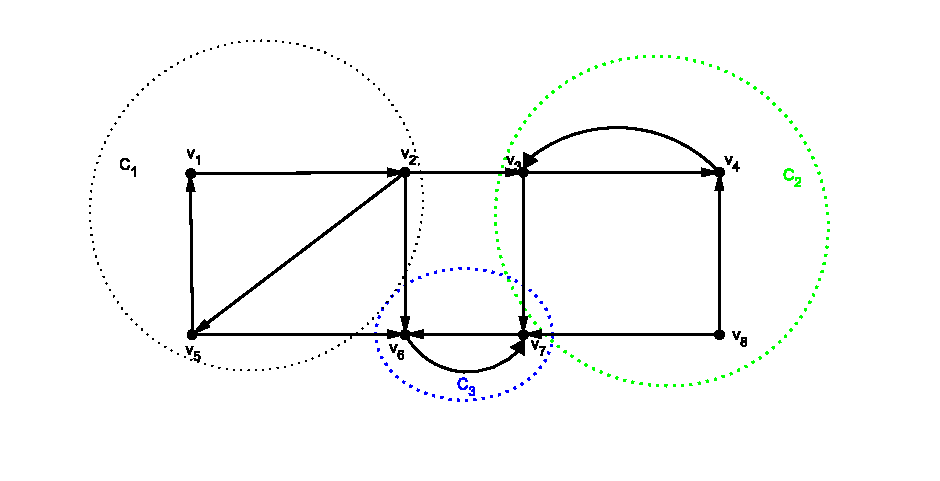
\includegraphics[scale=0.6]{componentes_conexa.eps}
\caption{$C_1$, $C_2$ y $C_3$ son componentes conexas de $D$}
\label{figura1}
\end{figure}


Una \emph{componente conexa} de una digr\'afica $D$ es una subdigr\'afica inducida maximal de $D$ que es fuertemente conexa. \\

%**************%**************%**********************%**********************%**************************

\chapter{Generalizaciones de n\'ucleos en digr\'aficas $m$-coloreadas con clases crom\'aticas cuasi-transitivas}

\section{La cerradura de una digr\'afica} 

Sea $D = (V,A)$ una digr\'afica $m$-coloreada. Definamos por $\mathcal{C}(D)$ a la digr\'afica cerradura de $D$. $\mathcal{C}(D)$ es tal que su conjunto de v\'ertices es el mismo que el de $D$ y tal que su conjunto de flechas, adem\'as de contener las mismas flecahs que $D$, por cada trayectoria monocrom\'atica en $D$ existe una flecha en $\mathcal{C}(D)$.

\begin{lemx}
Sea $D$ una digr\'afica m-coloreada. Supongamos que cada clase crom\'atica en $D$ es cuasi-transitiva. Si $C_k$ es un ciclo dirigido en ${Asym(\mathcal{C}(D)}$, entonces $C_k$ es un ciclo dirigido en \emph{Asym(D)}. 	
\end{lemx}

\begin{proof}

Sea $C_k = (x_1, x_2, \ldots, x_{k-1})$ un ciclo dirigido asim\'etrico en la cerradura de $D$. Notemos primero que, para que $C_k$ sea asim\'etrico, es necesario que exista al menos una flecha en $C_k$ que sea de distinto color que las dem\'as. Supongamos que el ciclo es monocrom\'atico. Para cualquier flecha del ciclo, por ejemplo para $(u_1,u_2)$, la $u_{2}u_{1}$-trayectoria $(u_2, u_3, \ldots, u_{k-1},u_k,u_1)$ est\'a en $D$. Entonces la flecha $(u_2,u_1)$ est\'a en $\mathcal{C}(D)$, lo que contradice que $C_k$ es asim\'etrico 

	\begin{figure} [ht]
	\centering
	\includegraphics[scale=0.5]{c_k_1.eps}
	\caption{$C_k$ est\'a en $D$}
	\label{figura1}
	\end{figure}

Tomemos una de las flechas de $C_k$, digamos $a=(x_i,x_{i+1})$. El caso en el que todas las flechas de $C_k$ est\'an en $D$ no necesita explicaci\'on, as\'i que consideremos el caso en el que $a$ no es flecha de $D$. Si $a$ no es flecha de $D$, debe existir en $D$ una $x_{i}x_{i+1}-$trayectoria monocrom\'atica. Recordemos que esta flecha es asim\'etrica ya que $C_k$ es un ciclo asim\'etrico.\\

Sea $P$ la $x_{i}x_{i+1}$-trayectoria monocrom\'atica en $D$ que da lugar a la existencia de $a$ en $\mathcal{C}(D)$. Supongamos que $P$ es minimal. Por hip\'otesis, cada clase crom\'atica en $D$ es cuasi-transitiva, y como $P$ es monocrom\'atica, podemos utilizar el resultado de la Proposici\'on 1.1. Notemos que, aunque $a$ es una flecha en $\mathcal{C}(D)$, hemos supuesto que $a$ no es una flecha de $D$. As\'i que descartamos el caso en el que la gr\'afica inducida de $P$ es semi-completa, ya que por ser $C_k$ un ciclo asim\'etrico, y $a$ una flecha en $C_k$, es imposible que exista la flecha $a' = (x_{i+1},x_i)$ en $D$, porque existir\'ia en $\mathcal{C}(D)$, haciendo sim\'etrica a $a$. \\

	\begin{figure} [ht]
	\centering
	\includegraphics[scale=0.5]{c_k_2.eps}
	\caption{$C_k$ est\'a en $D$}
	\label{figura1}
	\end{figure}

Entonces el orden de $P$ debe ser 4. Deben existir, dos v\'ertices $v_1,v_2$, distintos de $x_i$ y $x_{i+1}$ en $D$, tales que $(x_{i+1},v,u,x_i)$ es una trayectoria monocrom\'atica del mismo color que $P$. La trayectoria $(x_{i+1}, v_2, v_1, x_i)$ de longitud 2 est\'a en $D$, as\'i que existe en $\mathcal{C}(D)$ la flecha $a'=(x_{i+1},x_i)$. Esto hace a la flecha $a$, que pertenece al ciclo asim\'etrico $C_k$, sim\'etrica, lo cual es imposible. 

	\begin{figure} [ht]
	\centering
	\includegraphics[scale=0.5]{c_k_3.eps}
	\caption{$C_k$ est\'a en $D$}
	\label{figura1}
	\end{figure}


Por lo tanto, no es posible que exista una flecha en $C_k$ que no est\'e en $D$ como quer\'iamos probar. 

\end{proof}

\section{N\'ucleos por trayectorias monocrom\'aticas} 

En la secci\'on anterior presentamos los conceptos de independencia y dominaci\'on de un conjunto de v\'ertices de una digr\'afica. Ahora vamos a dar una generalizaci\'on deestos conceptos, utilizando como criterio la existencia de trayectorias monocrom\'aticas en lugar de flechas entre dos v\'ertices.\\

Sea $D = (V, A)$ una digr\'afica. Sea $K \subset V$. Decimos que $K$ es un \emph{conjunto independiente} de V, si para cualesquiera $u,v\in K$ no existe ni $(u,v)$  ni $(v,u) \in A$. Si cada v\'ertice que no est\'a en $K$ es absorbido por un v\'ertice en K decimos que K es un \emph{conjunto absorbente} de v\'ertices. Si $K$ es independiente y dominante decimos que $K$ es un \emph{n\'ucleo} de $D$.\\ 

\begin{teox}
Si cada ciclo dirigido de una digr\'afica $D$ tiene una flecha sim\'etrica, entonces $D$ es kernel-pefecta.
\end{teox} 

\begin{corox}
$D$ tiene un n\'ucleo por trayectorias monocrom\'aticas si y solo si $\mathcal{C}(D)$ tiene un n\'ucleo.
\end{corox}

\begin{proof}
Sea $K$ un n\'ucleo por trayectorias monocrom\'aticas de $D$. \\
$K$ es independiente por trayectorias monocrom\'aticas, entonces para cualesquiera dos v\'ertices $u, v$, no existe una uv-trayectoria, luego $(u,v)\notin A(D)$. Por lo tanto $K$ es independiente. $K$ es dominante por trayectorias monocrom\'aticas. Sea $u\in K$, para cierto v\'ertice $x \notin K$ existe la trayectoria $u \leadsto_{m} x \in D$. Luego la flecha $(u,x)$ est\'a en $\mathcal{C}(D)$. Por lo tanto $K$ es dominante en $\mathcal{C}(D)$.\\ 
Por lo tanto, $K$ es un n\'ucleo de $\mathcal{C}(D)$. \\ 
Sea $K$ un n\'ucleo de $\mathcal{C}(D)$.\\
$K$ es independiente en $\mathcal{C}(D)$. Para todo par de v\'ertices $u,v \in K$ no existe una flecha $(u,v)\in A(\mathcal{C}(D))$. Luego no existe una $uv-$trayectoria monocrom\'atica. Por lo tanto K es independiente por trayectorias monocrom\'aticas en D. $K$ es dominante en $\mathcal{C}(D)$. Para todo v\'ertice x $\notin K$, existe un v\'ertice $v \in K$ tal que $(v,u) \in A(\mathcal{C}(D))$, entonces existe una $vu$-trayectoria en $D$, luego $K$ es dominante por trayectorias monocrom\'aticas. \\
Por lo tanto $K$ es un n\'ucleo por trayectorias monocrom\'aticas de $D$.   
\end{proof}

\section{Resultados}
\begin{teox} Sea $D  = (V,F)$ una digr\'afica m-coloreada sin tri\'angulos policrom\'aticos. Supongamos que cada ciclo $C_k \in D$ es cuasi-transitivo en el borde y que cada clase crom\'atica es cuasi-transitiva. \\
\end{teox}
Sea $C_k = (u_1,u_2, \ldots, u_{k-1}, u_0)$ un c\'iclo asim\'etrico dirigido en $\mathcal{C}(D)$ de longitud m\'inima. Supongamos que $C_k$ es monocrom\'atico. Debido al Lema 2.1, sabemos que como $C_k$ es un c\'iclo asim\'etrico en $\mathcal{C}(D)$, y cada clase crom\'atica en $D$ es cuasi-transitiva, entonces $C_k$ es un ciclo en $D$. \\
	\begin{figure} [ht]
	\centering
	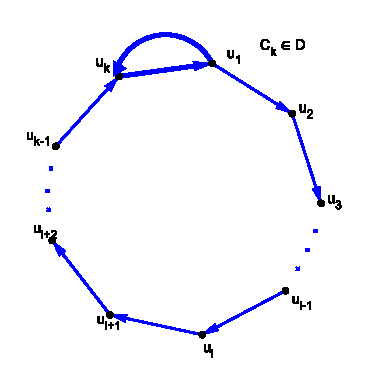
\includegraphics{figura1.eps}
	\caption{$C_k$ est\'a en $D$}
	\label{figura1}
	\end{figure}
La $u_2u_1$-trayectoria monocrom\'atica $M = (u_1, u_2, \ldots, u_{k-1}, u_1)$ est\'a en $D$ ya que todas sus aristas est\'an en $C_k$. La existencia de $M$ en $D$ nos garantiza que la flecha $(u_2,u_1)$ est\'a en $\mathcal{C}(D)$. Sin embargo, sabemos que la flecha $(u_1,u_2)$ en $C_k$ est\'a en $D$. Por lo tanto la flecha $[u_i,u_2]$ es sim\'etrica. Esto es imposible, $C_k$ es asim'etrico y por lo tanto todas sus flechas debe ser asim\'etricas. As\'i que existe un v\'ertice en $C_k$, digamos $u_i$, tal que el ciclo cambia de color, digamos de Azul a Rojo. Es decir, las flechas distintas a $(u_i, u_{i+1})$ en $C_k$ son de color Azul, y la flecha $(u_i,u_{i+1})$ es de color Rojo. \\
   Recordemos que $D$ es cuas-itransitiva en el borde. La trayectoria de longitud dos $(u_{i-1}, u_i, u_{i+1})$ en $C_k$ induce la existencia de una (y solo una) de las flechas $(u_{i-1},u_{i+1})$ y ($(u_{i+1},u_{i-1})$ en $D$. Sin embargo, el hecho de que $C_k$ sea asim\'etrico y cuasi-transitivo, junto con el cambio de color de las flechas en $u_i$ impide la existencia de $(u_{i+1},u_{i-1})$ en $\mathcal{C}(D)$. Analicemos los casos posibles. \\
		   El Lema 2.1 nos garantiza que el ciclo $C_k$ est\'a en $Asym(D)$, osea que todas sus flechas son asim\'etricas.. Supongamos que $(u_{i+1}, u_{i-1})$ est\'a en $D$. Se forma el ciclo $(u_{i-1},u_i,u_{i+1})$ en $D$ que por hip\'ostesis no puede ser policrom\'atico, as\'i que esta flecha no puede ser Verde. \\
		   Si $(u_{i+1},u_{i-1})$ fuera de color Azul, la trayectoria monocrom\'atica $(u_{i+1},u_{i-1},u_i)$, induce la existencia de $(u_{i+1},u_i)$ en $\mathcal{C}(D)$, ya que todas las clases crom\'aticas son cuasi-transitivas y la flecha entre $u_i$ y $u_{i+1}$ es sim\'etrica. Esto es imposible ya que $C_k$ es asim\'etrico. \\

	\begin{figure} [ht]
    \begin{minipage}[b]{0.5\linewidth}
	\centering
	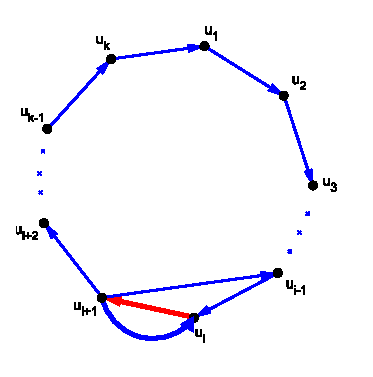
\includegraphics{figura2.eps}
	\caption{La flecha entre $u_{i-1}$ y $(u_{i+1})$ es sim\'etrica en $D$}
	\label{figura2}
	\end{minipage}
	\hspace{0.5cm}
	\begin{minipage}[b]{0.5\linewidth}
    \centering
	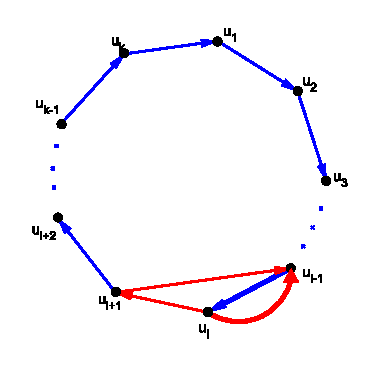
\includegraphics{figura3.eps}
	\caption{La flecha entre $u_{i+1}$ y $(u_i)$ es sim\'etrica en $D$}
	\label{figura3}
	\end{minipage}
	\end{figure}


		   An\'alogamente, si $(u_{i+1},u_{i-1})$ fuera de color Rojo, tenemos la trayectoria de longitud monocrom\'atica $(u_{i-1},u_{i+1},u_i)$, entonces $(u_{i-1},u_i)$ est\'a en $\mathcal{C}(D)$, haciendo sim\'etrica la flecha entre $u_{i-1}$ y $u_i$, ambos v\'ertices en el ciclo asim\'etrico $C_k$, esto tambi\'en es una contradicci\'on.  
		   	
	
		 %  Hemos probado que la flecha $(u_{i+1},u_{i-1})$ no puede ser de color Azul ni Rojo ni de ning\'un otro color distinto a estos dos, esta flecha no est\'a en $D$. Por lo tanto, $(u_{i-1},u_{i+1})$ es una flecha de $D$. \\ 
		  % $C_k$ es un ciclo asim\'etrico de longitud m\'inima. Probamos que $(u_{i-1},u_{i+1})$ es una flecha de $D$, y (por definici\'on) tambi\'en es una flecha de $\mathcal{C}(D)$. Con esta flecha podr\'iamos construir un ciclo nuevo en $\mathcal{C}(D)$ que no pasara por $u_i$, y por consecuencia, ser\'ia de menor longitud. Esto evidentemente contradice nuestra hip\'otesis de minimalidad sobre $C_l$. Vamos a probar que la flecha $(u_{i+1},u_{i-1})$ est\'a en $\mathcal{C}(D)$, lo que har\'ia la flecha entre estos v\'ertices sim\'etrica. Siendo as\'i, $(u_{i-1},u_{i+1})$ no puede formar parte de ning\'un ciclo asim\'etrico en $D$, y por lo tanto no es una flecha de $C_k$. Anteriormente probamos que la flecha $(u_{i+1},u_{i-1})$ no est\'a en $D$, sin embargo, $\mathcal{C}(D)$ tiene mas flechas que $D$, a saber, las flechas inducidas por cada trayectoria monocrom\'atica en $D$. \\
		   %Sea $C' = (u_0,u_1,\ldots,u_{i-1},u_{i+1},\ldots,u_{k-1},u_k)$ en $\mathcal{C}(D)$. Notemos que, salvo $(u_{i-1},u_{i+1})$, todas las flechas en $C'$ son flechas de $C_k$. Recordemos que cada una de estas flechas es asim\'etrica. Si $(u_{i-1},u_{i+1})$ fuera tambi\'en asim\'etrica, $C'$ ser\'ia un ciclo asim\'etrico de longitud menor a $k$, lo que contradice la minimalidad de $C_k$ en $Asym(\mathcal{C}(D))$. Por lo tanto, forzosamente la flecha entre $u_{i-1}$ y $u_{i+1}$ es sim\'etrica en $\mathcal{C}(D)$. Como ya hemos visto, en la digr\'afica cerradura $\mathcal{C}(D)$, existe una flecha por cada trayectoria monocrom\'atica en $D$. Por lo tanto, existe una $u_{i+1}u_{i-1}-$trayectoria monocrom\'atica en $D$, como consecuencia de la existencia de la flecha $(u_{i+1},u_{i-1})$ en $\mathcal{C}(D)$. Esta trayectoria en $D$ (que tambi\'en est\'a en $\mathcal{C}(D)$) tiene que ser de color Verde. Veamos por que: \\ 
	Hemos probado que la flecha $(u_{i+1},u_{i-1})$ no puede ser de color Azul ni Rojo ni de ning\'un otro color distinto a estos dos, entonces esta flecha no puede estar en $D$.Por lo tanto, $(u_{i-1},u_{i+1})$ est\'a en $D$. $C_k$ es un ciclo asim\'etrico de longitud m\'inima. Probamos que $(u_{i-1},u_{i+1})$ es una flecha en $D$ y por lo tanto una flecha en $\mathcal{C}(D)$. Con esta flecha podr\'iamos formar un ciclo nuevo en $\mathcal{C}(D)$ que no pasara por $u_i$, y por consecuencia, ser\'ia de menor longitud. Esto evidentemente contradice nuestra hip\'otesis de minimalidad sobre $C_k$. Sea $C' = (u_0,u_1,\ldots,u_{i-1},u_{i+1},\ldots,u_{k-1},u_k)$ un ciclo en $\mathcal{C}(D)$. Todas las flechas en $C'_k$, salvo $(u_{i-1},u_{i+1})$ son flechas tambi\'en en $C_k$, y por ende son asim\'etricas. Si $(u_{i-1},u_{i+1})$ fuera tambi\'en asim\'etrica, $C'$ ser\'ia un ciclo de longitud menor que $C_k$ en $Asym(\mathcal{C}(D)$. Esto es imposible, por lo tanto, la flecha entre $(u_{i-1}$ y $u_{i+1})$ debe ser sim\'etrica, osea $(u_{i+1},u_{i-1})$ es una flecha en $\mathcal{C}(D)$. Como acabamos de probar que esta flecha no est\'a en $D$, tiene que existir como consecuencia de la existencia de una trayectoria monocrom\'atica en $D$, recordemos que, en $\mathcal{C}(D)$ est\'an todas las flechas de $D$ y adem\'as hay una flecha por cada trayectoria monocrom\'atica en $D$ de ese color.  \\ 
		Llamemos $P$ a esta trayectoria. $P$ es del mismo color que $(u_{i+1},u_{i-1})$ y tiene que ser distinto de Rojo o Azul:\\
\begin{itemize}
\item{Si $(u_{i+1},u_{i-1})$ fuera Azul, la $u_{i-1}u_i$-trayectoria Azul se forma en $D$, y por ende la flecha $(u_{i+1},u_i)$ est\'a en $\mathcal{C}(D)$, ya que cada clase crom\'atica es cuasi-transitiva. La flecha $(u_i,u_{i+1})$ tambi\'en est\'a en $\mathcal{C}(D)$ pues es una flecha de $C_k$. Por lo tanto la flecha entre $u_i$ y $u_{i+1}$ es sim\'etrica, pero esto es imposible ya que supusimos que $(u_i,u_{i+1})$ est\'a en $C_k$, un ciclo asim\'etrico}
\item{Si esta flecha fuera Roja, haciendo un an\'alisis similar al anterior, tendr\'iamos la trayectoria monocrom\'atica $(u_i,u_{i+1},\ldots,u_{i-1})$ de color Rojo, luego, $(u_i,u_{i-1})$ es una flecha en $\mathcal{C}(D)$, entonces la flecha entre $u_{i-1}$ y $u_i$, ambos v\'ertices en $C_k$, es sim\'etrica en $\mathcal{C}(D)$, lo que contradice la asimetricidad de $C_k$}
\end{itemize}

Entonces $P$ es una trayectoria monocrom\'atica Verde en $D$. Supongamos que el v\'ertice en $C_k$ $u_i$ est\'a en $P$. Entonces la $u_{i+1}u_i$-trayectoria monocrom\'atica en $D$ garantiza la existencia de la flecha $(u_{i+1},u_i)$ en $\mathcal{C}(D)$, haciendo sim\'etrica a la flecha entre $u_i$ y $u_{i+1})$, que es una flecha en $C_k$ un ciclo asim\'etrico, esto nos lleva a una contradicci\'on. Por lo tanto $u_i$ no es uno de los v\'ertices en $P$. \\ 
	A continuaci\'on vamos a probar uqe dada una digr\'afica $D$ sin tri\'angulos policrom\'aticos, y con todos sus ciclos cuasi-transitivos y cada clase crom\'atica cuasi-transitiva, cada ciclo dirigido en $\mathcal{C}(D)$ tiene una flecha sim\'etrica. Si sucede esto sabemos, debido a Teorema 2.2, que $\mathcal{C}(D)$ es kernel-perfecta. Debido al Corolario 2.3 sabremos que $D$ tiene un n\'ucleo por trayectorias monocrom\'aticas. \\ 
	\begin{teox}
	Sea $D = (V,F)$ una digr\'afica m-coloreada sin tri\'angulos policrom\'aticos. Supongamos que cada ciclo $C_k$ en $D$ es cuasi-transitivo en el borde, y que cada clase crom\'atica es cuasi-transitiva. Entonces $D$ tiene un n\'ucleo por trayectorias monocrom\'aticas. 
	\end{teox}

	Sea $C_k = (u_1,u_2,\ldots,u_{k-1},u_0)$ un ciclo dirigido en $Asym(\mathcal{C}(D)$. Por hip\'otesis no existen tri\'angulos policrom\'aticos en $D$, esto evidentemente incluye a los ciclos de longitud 3, siendo as\'i, se cumplen las hip\'otesis del Teorema 2.5 y podemos afirmar lo siguiente: 
			\begin{itemize}
			\item{Existe un v\'ertice $u_i$ en $C_k$, tal que todas las flechas en el ciclo son de color Azul y $(u_i,u_{i+1})$ es de color Rojo}
			\item{$(u_{i-1}, u_{i+1})$ est\'a en $D$}
			\item{$(u_{i+1},u_{i-1})$ no es una flecha en $D$, $(u_{i+1},u_{i-1})$ si una flecha en $\mathcal{C}(D)$, y por lo tanto existe $P$, una $u_{i+1}u_{i-1}-$trayectoria en $D$, de color Verde}
			\item{$u_i$ no es un v\'ertice de $P$}
			\end{itemize}

			Supongamos sin p\'erdida de generalidad que $P$ es de longitud m\'inima. La clase crom\'atica verde es cuasi-transitiva por hip\'otesis. La flecha $(u_{i-1},u_{i+1})$ no est\'a en la clase crom\'atica del Verde pues $D$ no contiene tri\'angulos policrom\'aticos, recordemos que $P$ es Verde. Se cumplen las hip\'otesis que nos garantizan en virtud de la Proposici\'on 1.2, que la longitud de la trayectoria debe ser 4 y que existen v\'ertices $v_1,v_2$ en $D$ distintos a $u_{i+1}$ y a $u_{i-1})$ tales que las trayectorias dirigidas $(u_{i+1},v_2,v_1,u_{i-1})$ y $(u_{i-1},v_1,v_2,u_{i+1})$ est\'an en $D$. Con estas aristas podemos formar el ciclo $(u_i,u_{i+1},v_1,v_2,u_{i-1},u_i)$. Como todos los ciclos en $D$, es cuasi-trasntivio en el borde por hip\'otesis, as\'i que debe existir una flecha entre $u_i$ y $v_2$ en $D$, como consecuencia de que la trayectoria de longitud dos $(u_i,u_{i+1},v_1)$ est\'a en $D$. \\ 
	Supongamos que $(u_i,v_1)$ es una flecha de $D$.
	Si fuera Verde la flecha entre $u_{i-1}$ y $u_i$ estar\'ia en $\mathcal{C}(D)$ contradiciendo la asimetricidad de $C_k$. \\
	Si esta flecha fuera de un color distinto, tendr\'iamos los tri\'angulos policrom\'aticos $(u_i,v_1,u_{i+1})$ o $(u_i,v_1,u_{i-1})$ en $D$ lo cual tambi\'en contradice nuestras hip\'otesis. \\ 
	En resumen, Si $C_k$ fuera un ciclo asim\'etrico en $\mathcal{C}(D)$, $C_k$ tendr\'ia una flecha sim\'etrica, y por lo tanto $D$ ser\'ia kernel perfecta y debido al Teorema 2.2, sabemos que $D$ tiene un n\'ucleo por trayectorias monocrom\'aticas. \\ 
\end{document}

Fin.
\cleardoublepage %maybe this isn't needed

%%%%---------------------------------------------------------------------------------------------------------------
%   FINALE
%%%%---------------------------------------------------------------------------------------------------------------

\backmatter

%%%%---------------------------------------------------------------------------------------------------------------
%   CONCLUSION
%%%%---------------------------------------------------------------------------------------------------------------

\newpage 
\chapter{Conclusi�n}
Concluimos.
\clearpage\mbox{}\clearpage

%%%%---------------------------------------------------------------------------------------------------------------
%   APPENDIX
%%%%---------------------------------------------------------------------------------------------------------------

\appendix

%%%%---------------------------------------------------------------------------------------------------------------
%   SYMBOL LIST
%%%%---------------------------------------------------------------------------------------------------------------

\newpage
\addcontentsline{toc}{chapter}{�ndice de s�mbolos}
\printnomenclature[1.1in]

%%%%---------------------------------------------------------------------------------------------------------------
%   FIGURE LIST
%%%%---------------------------------------------------------------------------------------------------------------

\newpage
\addcontentsline{toc}{chapter}{�ndice de figuras}
\makeatletter \renewcommand{\@dotsep}{1000} \makeatother
\listoffigures

%%%%---------------------------------------------------------------------------------------------------------------
%   BIBLIOGRAPHY
%%%%---------------------------------------------------------------------------------------------------------------

\addcontentsline{toc}{chapter}{Bibliograf�a}
\begin{thebibliography}{20}
%\bibitem{label} \textsc{Author}, Title, \emph{Book} (YEAR) PageA-PageB.
\bibitem{articuloa} \textsc{A. Einstein}, F�sica, \emph{Libro A} (1700) 222-223.
\bibitem{articulob} \textsc{I. Newton}, Manzanas, \emph{Libro X} (1200) 490-2301.
\end{thebibliography}

%%%%---------------------------------------------------------------------------------------------------------------
%   BAD END
%%%%---------------------------------------------------------------------------------------------------------------

\end{document}
